\documentclass[compress]{beamer}
\usepackage{ifthen,verbatim}

\newcommand{\isnote}{}
\xdefinecolor{lightyellow}{rgb}{1.,1.,0.25}
\xdefinecolor{darkblue}{rgb}{0.1,0.1,0.7}
\xdefinecolor{darkgreen}{rgb}{0.1,0.6,0.1}

%% Uncomment this to get annotations
%% \def\notes{\addtocounter{page}{-1}
%%            \renewcommand{\isnote}{*}
%% 	   \beamertemplateshadingbackground{lightyellow}{white}
%%            \begin{frame}
%%            \frametitle{Notes for the previous page (page \insertpagenumber)}
%%            \itemize}
%% \def\endnotes{\enditemize
%% 	      \end{frame}
%%               \beamertemplateshadingbackground{white}{white}
%%               \renewcommand{\isnote}{}}

%% Uncomment this to not get annotations
\def\notes{\comment}
\def\endnotes{\endcomment}

\setbeamertemplate{navigation symbols}{}
\setbeamertemplate{headline}{\mbox{ } \hfill
\begin{minipage}{5.5 cm}
\vspace{-0.75 cm} \small
\end{minipage} \hfill
\begin{minipage}{4.5 cm}
\vspace{-0.75 cm} \small
\begin{flushright}
\ifthenelse{\equal{\insertpagenumber}{1}}{}{Jim Pivarski \hspace{0.2 cm} \insertpagenumber\isnote/\pageref{numpages}}
\end{flushright}
\end{minipage}\mbox{\hspace{0.2 cm}}\includegraphics[height=1 cm]{../cmslogo} \hspace{0.1 cm} \includegraphics[height=1 cm]{../tamulogo} \hspace{0.01 cm} \vspace{-1.05 cm}}

\begin{document}
\section*{Title and introduction}

\begin{frame}
\vfill
\begin{center}
\textcolor{darkblue}{\Large Track-based Alignment in CSA08 and CRUZET}

\vfill
\begin{columns}
\column{0.3\linewidth}
\begin{center}
\large
\textcolor{darkblue}{Jim Pivarski}

\vspace{0.2 cm}
Alexei Safonov
\end{center}

\column{0.3\linewidth}
\begin{center}
\large
K\'aroly Banicz
\end{center}
\end{columns}

\begin{columns}
\column{0.3\linewidth}
\begin{center}
\scriptsize
{\it Texas A\&M University}
\end{center}
\column{0.3\linewidth}
\begin{center}
\scriptsize
{\it US-CMS}
\end{center}
\end{columns}

\vfill
25 July, 2008

\end{center}
\end{frame}

%% \begin{notes}
%% \item This is the annotated version of my talk.
%% \item If you want the version that I am presenting, download the one
%% labeled ``slides'' on Indico (or just ignore these yellow pages).
%% \item The annotated version is provided for extra detail and a written
%% record of comments that I intend to make orally.
%% \item Yellow notes refer to the content on the {\it previous} page.
%% \item All other slides are identical for the two versions.
%% \end{notes}

\begin{frame}
\frametitle{Outline}
\begin{itemize}\setlength{\itemsep}{0.75 cm}
\item Monte Carlo studies of long-term procedure: CSA08 \hfill {\scriptsize \it \textcolor{darkblue}{(9~min)}}
\begin{itemize}
\item answered ``last'' basic questions about how the

procedure will perform with collisions data
\end{itemize}

\item Alignment of stations in CRUZET \hfill {\scriptsize \it \textcolor{darkblue}{(12~min)}}
\begin{itemize}
\item based on the long-term procedure
\item real data! production-quality results!
\item aligned constants make sense, agree with

external measurements
\end{itemize}

\item Chamber alignment with overlaps \hfill {\scriptsize \it \textcolor{darkblue}{(9~min)}}
\begin{itemize}
\item developing procedure for beam-halo sample
\item testing and debugging with CRUZET cosmic rays
\end{itemize}
\end{itemize}
\end{frame}

\section*{CSA08 Monte Carlo Studies}
\begin{frame}
\begin{center}
\Huge \textcolor{blue}{CSA08 Monte Carlo Studies}
\end{center}
\end{frame}

\begin{frame}
\frametitle{Goals for CSA08 exercise}
\small

\begin{itemize}
\item To demonstrate that
\begin{itemize}
\item our long-term procedure works in a realistic simulation
\item we can coordinate with other alignment/calibration groups in a timed test (1~week from ``data'' to constants)
\end{itemize}
\item To study effects that require huge MC samples in a recent release
\end{itemize}

\vfill
\hspace{-0.83 cm} \textcolor{darkblue}{\Large Parameters of the study}
\begin{itemize}
\item Long-term procedure: fit tracks to tracker as a reference, minimize residuals in muon chambers
\item Align individual chambers in barrel and endcap
\item 10~pb$^{-1}$ of inclusive muons, but no cosmic rays/beam-halo
\end{itemize}

\vspace{-0.3 cm}
\begin{center}
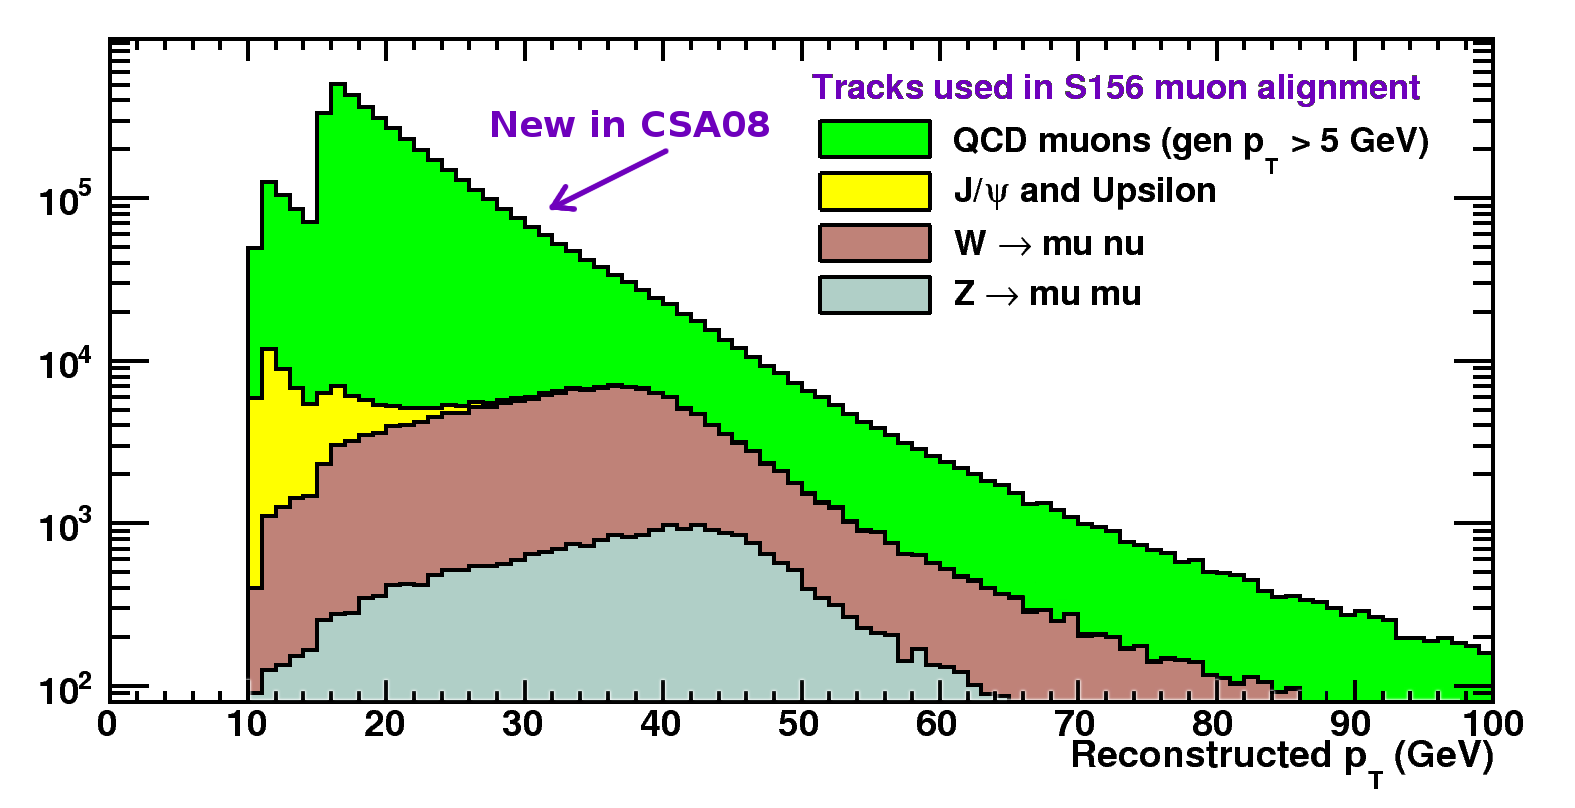
\includegraphics[width=0.6\linewidth]{S156_pt_spectrum_noQCD5.png}
\end{center}

\vspace{-0.8 cm}
\mbox{ }
\end{frame}

\begin{frame}
\frametitle{10~pb$^{-1}$ results at a glance}
\small
Histograms of aligned positions minus true positions in $r\phi$

MB1: 680~microns \hspace{0.3 cm} ME1/1: 520~microns \hspace{0.3 cm} ME1/2: 840~microns

\vfill
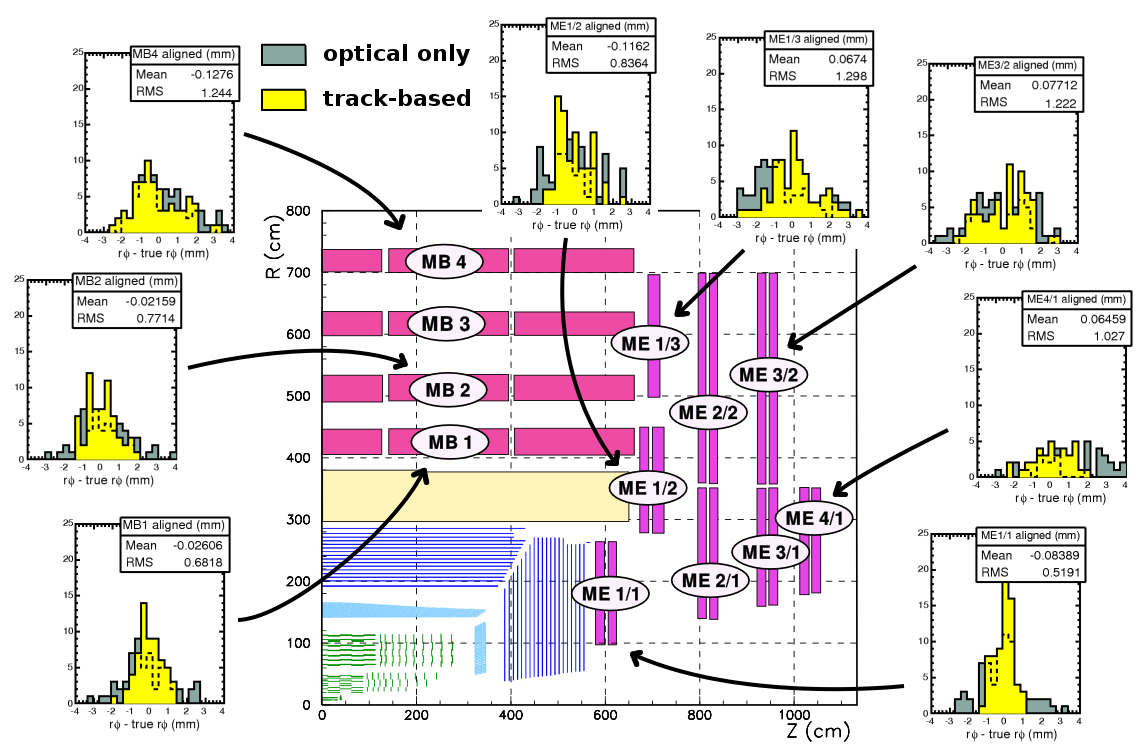
\includegraphics[width=\linewidth]{all_results_crop.png}
\end{frame}

\begin{frame}
\frametitle{Key result \#1}
\small

\hspace{-0.83 cm} \textcolor{darkblue}{\Large Strong dependence on tracker misalignment}

\vspace{-0.1 cm}
\begin{center}
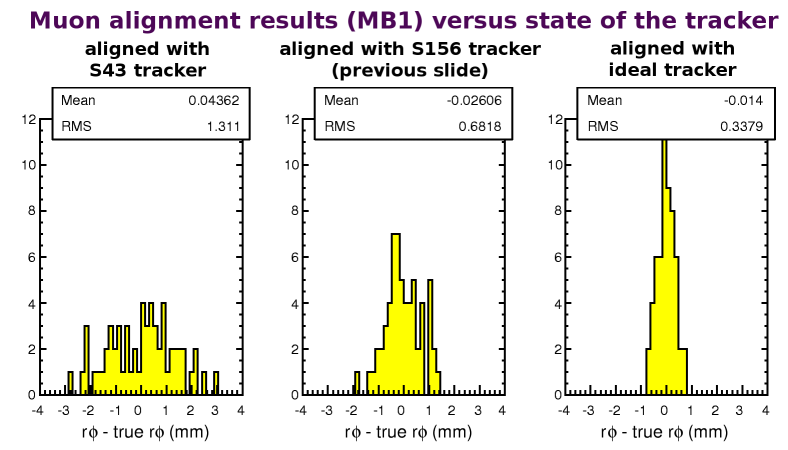
\includegraphics[width=0.7\linewidth]{muonalignment_MB1_dep_on_tracker.png}
\end{center}

\vspace{-0.25 cm} \renewcommand{\arraystretch}{0.6}
\begin{tabular}{p{0.45\linewidth} c | c p{0.45\linewidth}}
Previous studies used randomly-generated tracker misalignment scenarios & & & models internal misalignment

correlations expected from

assembly only \\

& & & \\\hline

& & & \\

New study uses output of tracker alignment algorithm as input to muon alignment & & & includes correlations generated by tracker alignment attempt:

we see more dependence

\end{tabular}

\end{frame}

\begin{frame}
\frametitle{Analysis of tracker dependence}
\small

\begin{itemize}
\item Alignment performed using tracks from the interaction point
\item Tracks that reach a given chamber all pass through the same narrow region of the tracker
\item Tracker misalignments are $\mathcal{O}(\mbox{10 $\mu$m})$, effect is 680~$\mu$m
\end{itemize}

Mismeasured $\phi$ or $\eta$: \hfill \mbox{$\displaystyle 10\mbox{ $\mu$m}\, \left(\frac{\mbox{4-6 m inner muon station}}{\mbox{1-2 m tracker radius/half-length}}\right) = 60\mbox{ $\mu$m}$ \hspace{-0.3 cm}}

\vspace{0.2 cm}
Mismeasured curvature: \hfill $\displaystyle 10\mbox{ $\mu$m}\, \left(\frac{\mbox{4 m inner muon station}}{\mbox{0.5 m tracker half-radius}}\right)^2 = 640\mbox{ $\mu$m}$

\vspace{0.2 cm}

\includegraphics[width=\linewidth]{dotted-line.pdf}

\vspace{-0.2 cm}
\begin{center}
\hspace{0.5 cm} \scriptsize Why curvature error is quadratic in lever arm: \hfill \mbox{ }

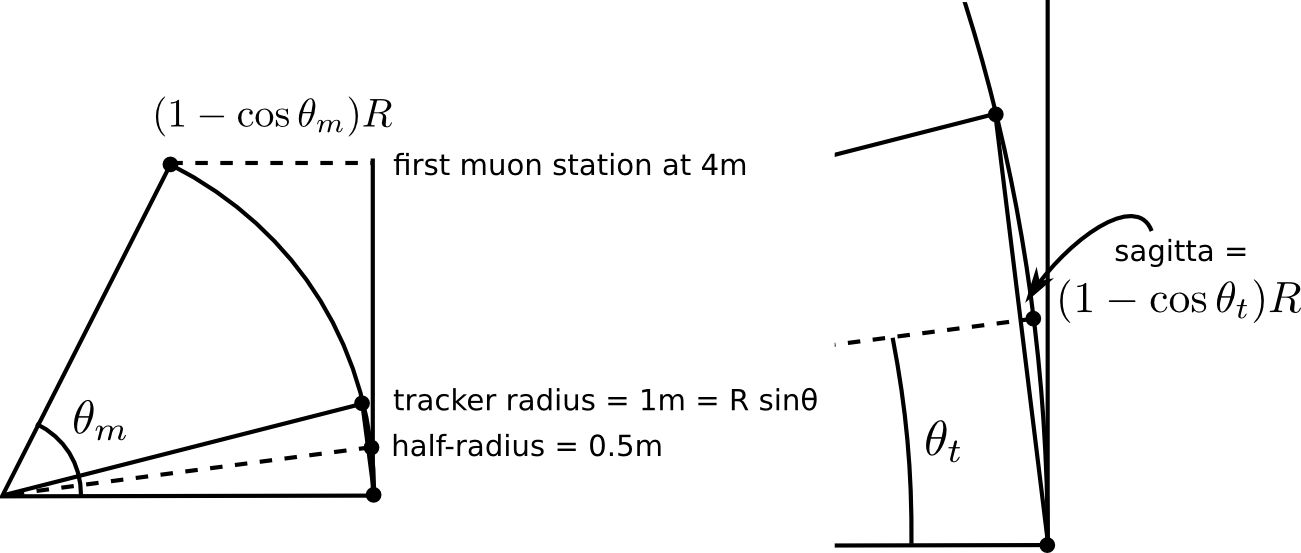
\includegraphics[width=0.7\linewidth]{curvature_extrapolation.png}
\end{center}
\end{frame}

\begin{frame}
\frametitle{Solutions}

\begin{center}
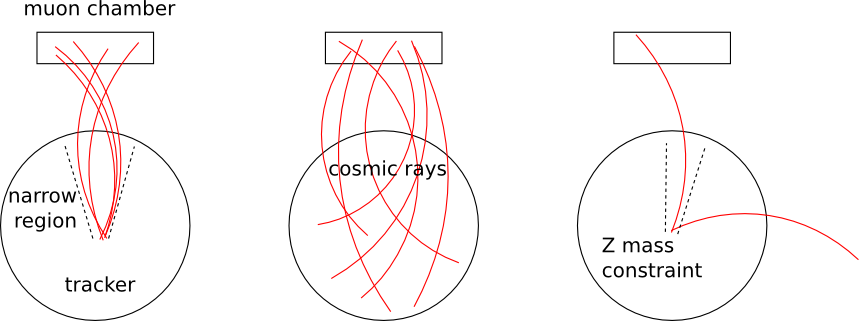
\includegraphics[width=0.8\linewidth]{solutions.png}
\end{center}

\vfill
We need to ``average over'' the tracker more, so that a muon chamber isn't always seeing tracks mismeasured in the same narrow region

\begin{itemize}
\item \textcolor{darkblue}{\fbox{Easiest and possibly best: align with cosmic rays}}
\item With 100~pb$^{-1}$ or more: constrain $Z\to\mu\mu$ to mix momentum measurements from different regions
\item Discussed possibility of using lever arm from muon system to improve tracker alignment
\end{itemize}
\end{frame}

\begin{frame}
\frametitle{Key result \#2}
\small

\textcolor{darkblue}{Long-standing question:} is it better\ldots
\begin{itemize}
\item to select high-momentum tracks and reduce multiple scattering (minimize standard deviation of residuals)
\item or open the floodgates and let in all muons (maximize $\sqrt{N}$)?
\end{itemize}

\vfill
Alignment correction is (roughly) mean of residual distribution,
\[ \mbox{uncertainty} = \frac{\mbox{standard deviation}}{\sqrt{N}} \]

\vfill
\textcolor{darkblue}{Answer:} open the floodgates (minimum $p_T$ of 10~GeV)

\vspace{0.1 cm}
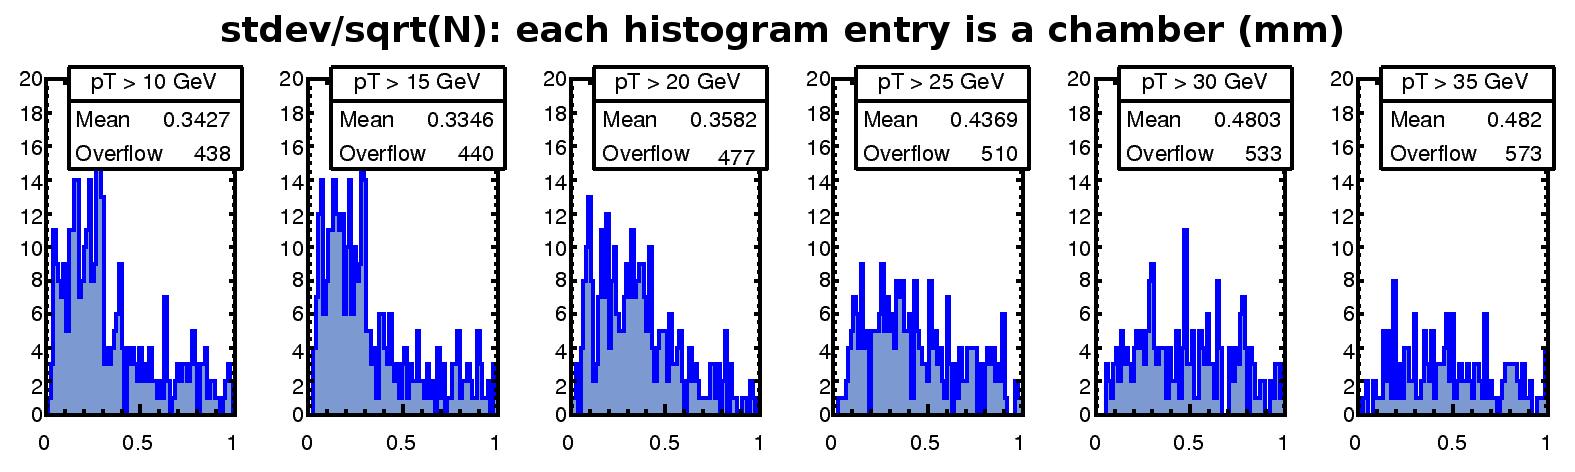
\includegraphics[width=\linewidth]{widening.png}
\end{frame}

\begin{frame}
\frametitle{Conclusions for CSA section}

\vfill
\begin{itemize}\setlength{\itemsep}{0.2 cm}
\item Long-term alignment procedure is ready for data
\item 10~pb$^{-1}$ $\approx$ all of 2008
\item Cosmic rays can improve upon this result
\item Makes an impact in benchmark $Z' \to \mu\mu$ analysis:
\end{itemize}

\vfill
\mbox{ } \hfill 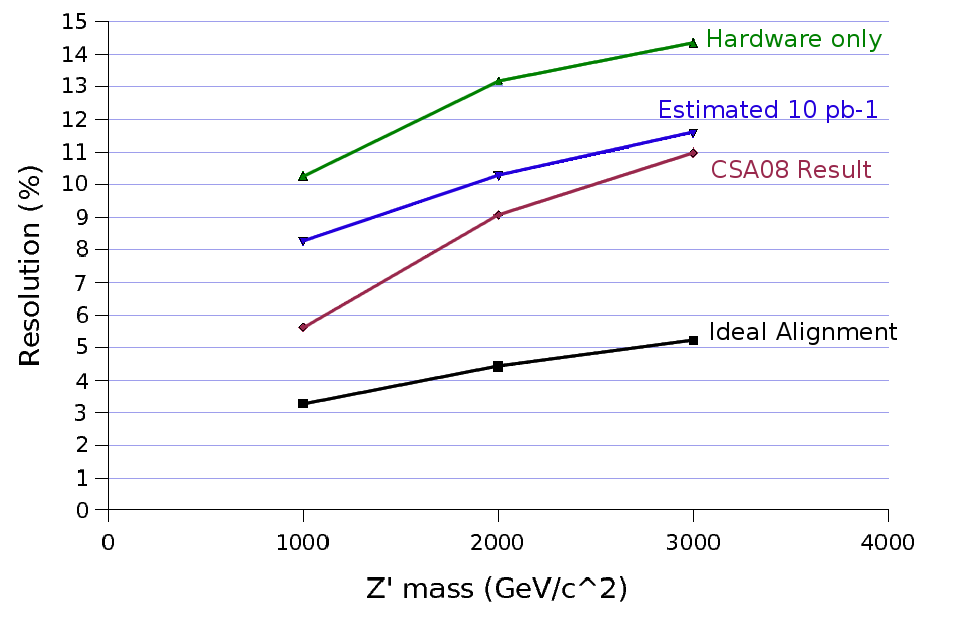
\includegraphics[width=0.7\linewidth]{z-prime.png} \hfill \mbox{ }

\end{frame}

\section*{Real Alignment of Stations}
\begin{frame}
\begin{center}
\Huge \textcolor{blue}{Real Alignment of Stations}
\end{center}
\end{frame}

\begin{frame}
\frametitle{Fix common coordinate system}

Largest and most important part of alignment: find out where the
stations are relative to the rest of CMS

\begin{itemize}
\item improves track residuals by many centimeters
\end{itemize}

\vfill
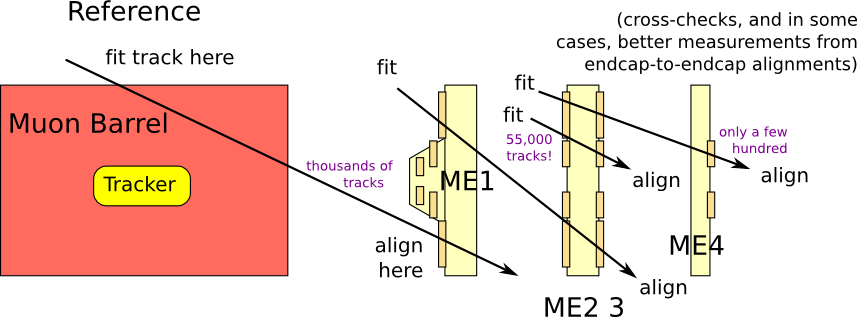
\includegraphics[width=\linewidth]{fit_here_align_there.png}

\vfill
Similar to the long-term procedure, except that the muon barrel is the
reference, rather than the tracker
\end{frame}

\begin{frame}
\frametitle{Aligning with HIP derivatives}
\small

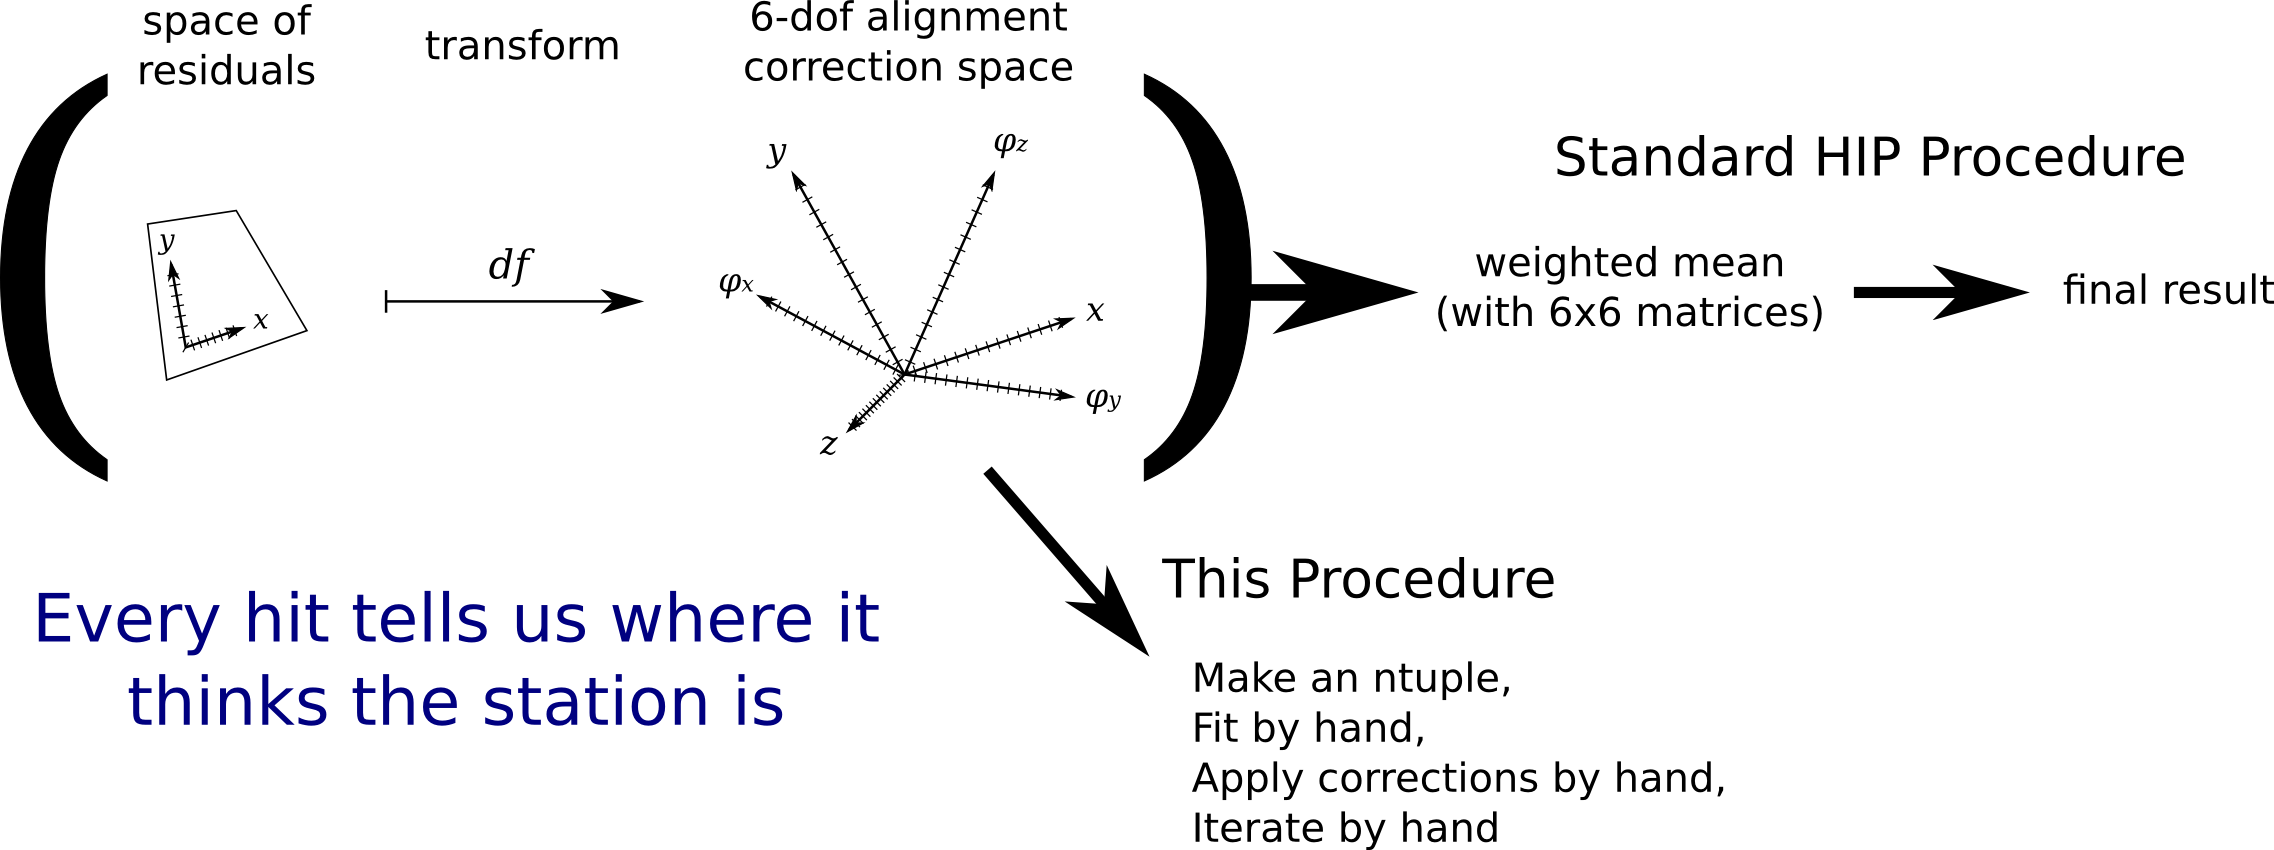
\includegraphics[width=\linewidth]{transformation.png}

\begin{columns}
\column{0.4\linewidth}
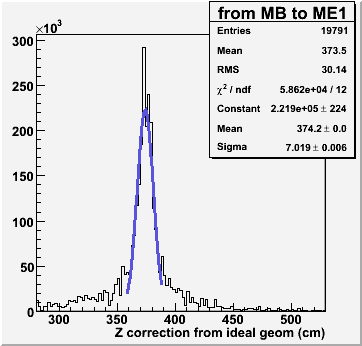
\includegraphics[width=\linewidth]{hist_0and1.png}

\column{0.65\linewidth}
Histogram of $z$ correction from every hit

\begin{itemize}
\item Without a magnetic field, can't cut on $p_T$
\item Bad tracks/hits form a broad distribution
\item Good tracks/hits agree on a $z$ position
\item Tape-measure agrees, too: 370~cm
\end{itemize}
\end{columns}
\end{frame}

\begin{frame}
\frametitle{Results at a glance:}
\vspace{-0.4 cm}
\hspace{-0.83 cm} \textcolor{darkblue}{\Large Where were our stations?}

\vfill
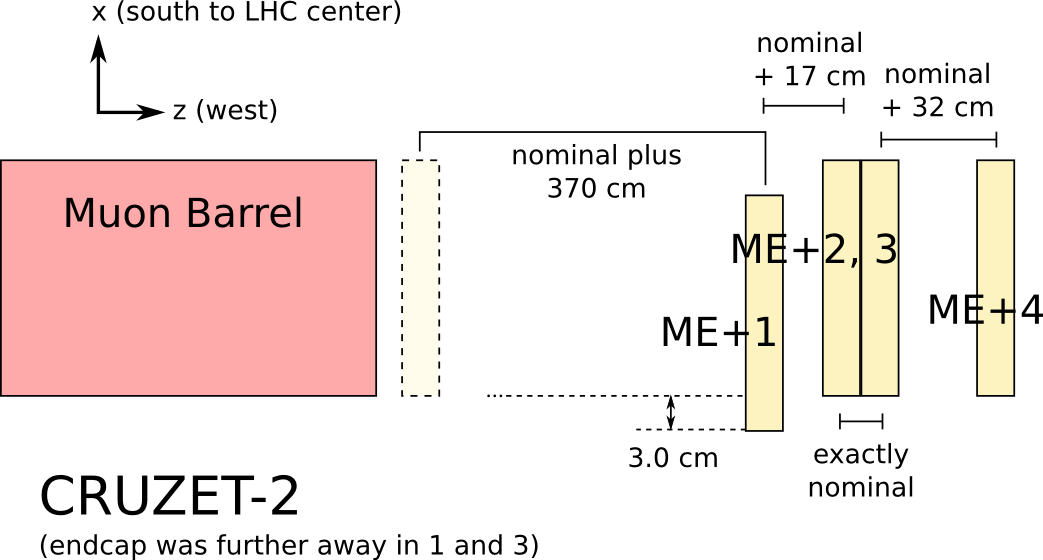
\includegraphics[width=\linewidth]{where_things_are.png}

\vfill
Constants are ready; will upload to database very soon
\end{frame}

\begin{frame}
\frametitle{Procedure details}

Best resolution in outer stations from leap-frog approach

``MB $\to$ 2 $\to$ 3'' means measure corrections between MB and ME2
and between ME2 and ME3, then add them

\begin{center}
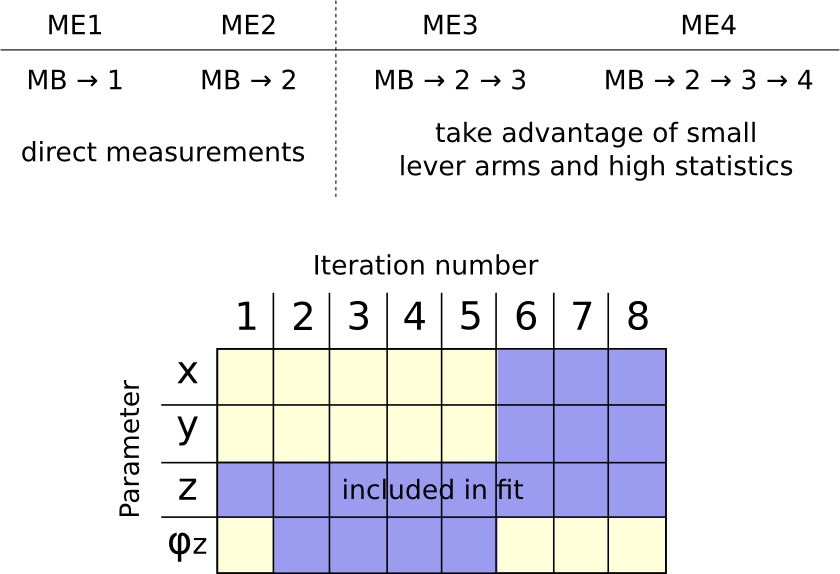
\includegraphics[width=0.7\linewidth]{stepping_stones.png}
\end{center}

\begin{itemize}
\item $\phi_x$ and $\phi_y$ are not additive, but also consistent with zero
\item $\phi_z$ becomes non-additive after applying $x$ and $y$ corrections
\end{itemize}
\end{frame}

\begin{frame}
\frametitle{Error analysis and consistency}
\small

Na\"ive uncertainty estimate: Gaussian width/$\sqrt{N}$
\begin{itemize}
\item $x$, $y$: 0.2--0.9~mm, but 0.03~mm in ME2 $\to$ 3 (high stats)
\item $z$: 0.3--1.6~mm, but 0.07~mm in ME2 $\to$ 3
\item $\phi_z$: 0.07--0.3~mrad, but 0.01~mrad in ME2 $\to$ 3
\end{itemize}

\vfill
Consistency checks
\begin{tabular}{c | c c c c}
\scriptsize Comparison & \scriptsize $x$ (mm) & \scriptsize $y$ (mm) & \scriptsize $z$ (mm) & \scriptsize $\phi_z$ (mrad) \\\hline
\scriptsize (MB$\to$2) $-$ (MB$\to$1$\to$2) & \scriptsize -12.8 $\pm$ 0.3 & \scriptsize 6.4 $\pm$ 0.4 & \scriptsize 39.9 $\pm$ 0.8 & \scriptsize -4.75 $\pm$ 0.12 \\
\scriptsize (MB$\to$3) $-$ (MB$\to$2$\to$3) & \scriptsize -3.4 $\pm$ 0.4 & \scriptsize -8.7 $\pm$ 0.5 & \scriptsize -15.3 $\pm$ 1.0 & \scriptsize -1.06 $\pm$ 0.14 \\
\scriptsize (MB$\to$4) $-$ (MB$\to$3$\to$4) & \scriptsize 0.4 $\pm$ 0.8 & \scriptsize 6.0 $\pm$ 0.9 & \scriptsize 10.3 $\pm$ 2.4 & \scriptsize 2.8 $\pm$ 0.3 \\\hline
\end{tabular}

\vfill
Statistics-only underestimates the error

\vfill
\[ \sqrt{\frac{1}{N-1} \sum (x_i - \bar{x})^2} = \left\{\begin{array}{l} \mbox{7.8~mm for $x$ and $y$} \\ \mbox{28~mm for $z$} \\ \mbox{3.8~mrad for $\phi_z$} \end{array}\right. \]

\vfill
But (MB $\to$ 2) and (MB $\to$ 3) are double-counted, so this is an
overestimate (and dominated by the worst stations)
\end{frame}

\begin{frame}
\frametitle{Cute observations}

\begin{itemize}\setlength{\itemsep}{0.3 cm}
\item Taking conservative $\sigma_{x,y}$ $\lesssim$ 7.8~mm, $-$30~mm shift in ME1 $x$ is significant

\item ME2 and ME3 are only 2.3 and 2.0~$\sigma$ underground

\item Experimentally ``discovered'' that ME2 and ME3 are mounted on the same yoke

\end{itemize}

\vspace{-0.5 cm}
\[ \left.\begin{array}{c c c} \Delta x &=& \mbox{1.3~mm} \\ \Delta y &=& \mbox{2.5~mm} \\ \Delta z &=& \mbox{0.1~mm} \\ \Delta \phi_z &=& \mbox{0.42~mrad} \end{array}\right\} \mbox{ very small or consistent with zero} \]

\vfill
Unusually small $\Delta z$, only possible if their alignments \mbox{are linked\hspace{-1 cm}}

\vfill
Blind analysis: I didn't know (we don't model this \mbox{relationship in MC)\hspace{-1 cm}}
\end{frame}

\begin{frame}
\frametitle{Individual chambers?}

Ultimately, we will want to align individual chambers with a method like this

\vfill
Can we test that now?

Unfortunately, no (few millimeters resolution in CRUZET-2)

\vspace{-2 cm}
\begin{columns}
\column{0.63\linewidth}
Determine collective radial position or $\phi_x$?

\begin{itemize}
\item Compute chamber-level corrections and merge histograms per station
\item Useful for following gross motion of station under $\vec{B}$
\end{itemize}

\column{0.4\linewidth}
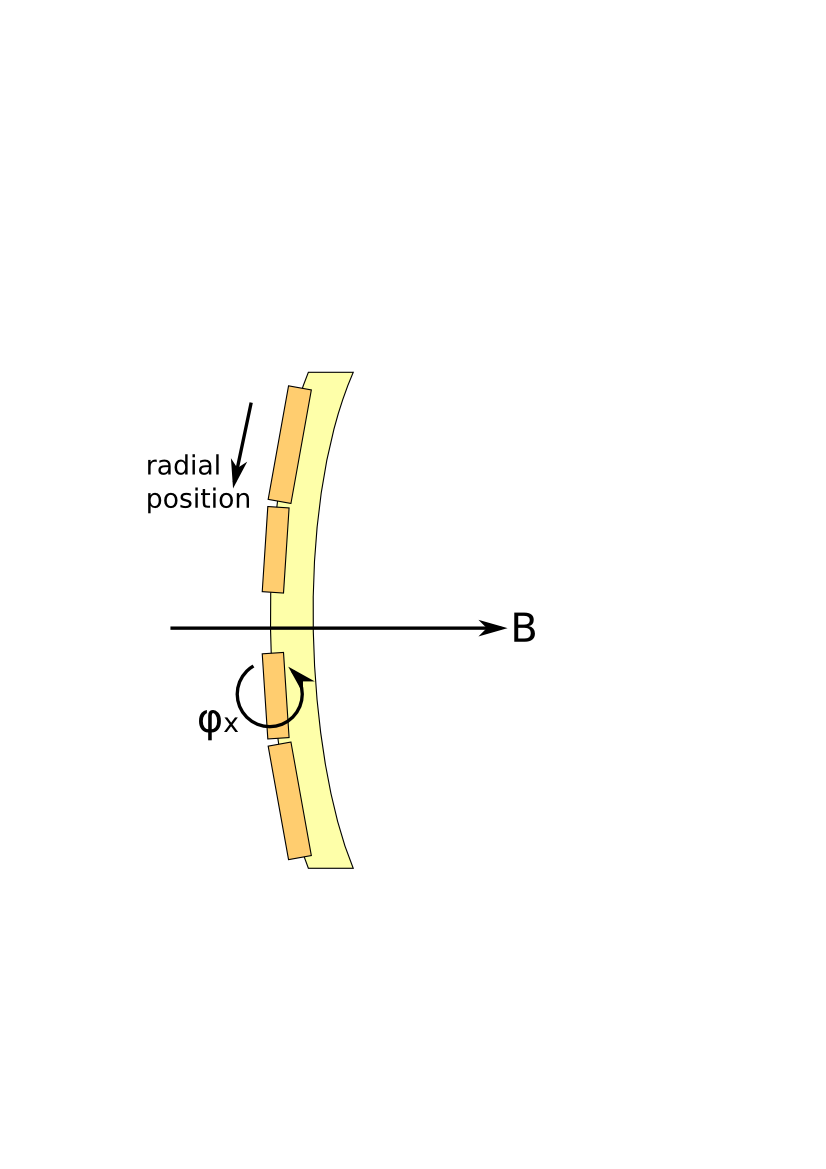
\includegraphics[width=1.2\linewidth]{turn_on_magnet.png}
\end{columns}

\vspace{-1.2 cm}
CRUZET-3 has $\sim$5 times the statistics and tracker may provide better-quality tracks
\end{frame}

\begin{frame}
\frametitle{Conclusions for station alignment}
\begin{itemize}\setlength{\itemsep}{0.75 cm}
\item Alignment converges and makes sense

\item Survives internal consistency checks at the level of 7.8~mm
  ($x$-$y$), 28~mm ($z$), and 3.4~mrad ($\phi_z$)

\item Non-Gaussian components in residuals identified as irreducible
  low-momentum tracks: right now, fitting is necessary

\item Worth noting: chamber-by-chamber histograms are more nearly Gaussian

\end{itemize}
\end{frame}

\section*{Alignment with Overlapping CSCs}
\begin{frame}
\begin{center}
\Huge \textcolor{blue}{Alignment with}

\textcolor{blue}{Overlapping CSCs}
\end{center}
\end{frame}

\begin{frame}
\frametitle{CSC-Overlaps alignment}

\begin{columns}
\column{0.8\linewidth}

Determine relative alignment of pairs of chambers using tracks that pass through both

\begin{itemize}
\item Very little multiple scattering; simple linear fit
\item Align CSC rings internally
\item Beam-halo events are ideal, cosmics will work
\item Compliments alignment of whole rings/disks from an external reference
\end{itemize}

\column{0.2\linewidth}
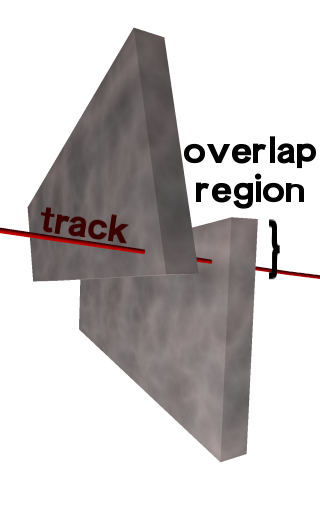
\includegraphics[width=\linewidth]{overlap.png}
\end{columns}

\vfill
\vfill
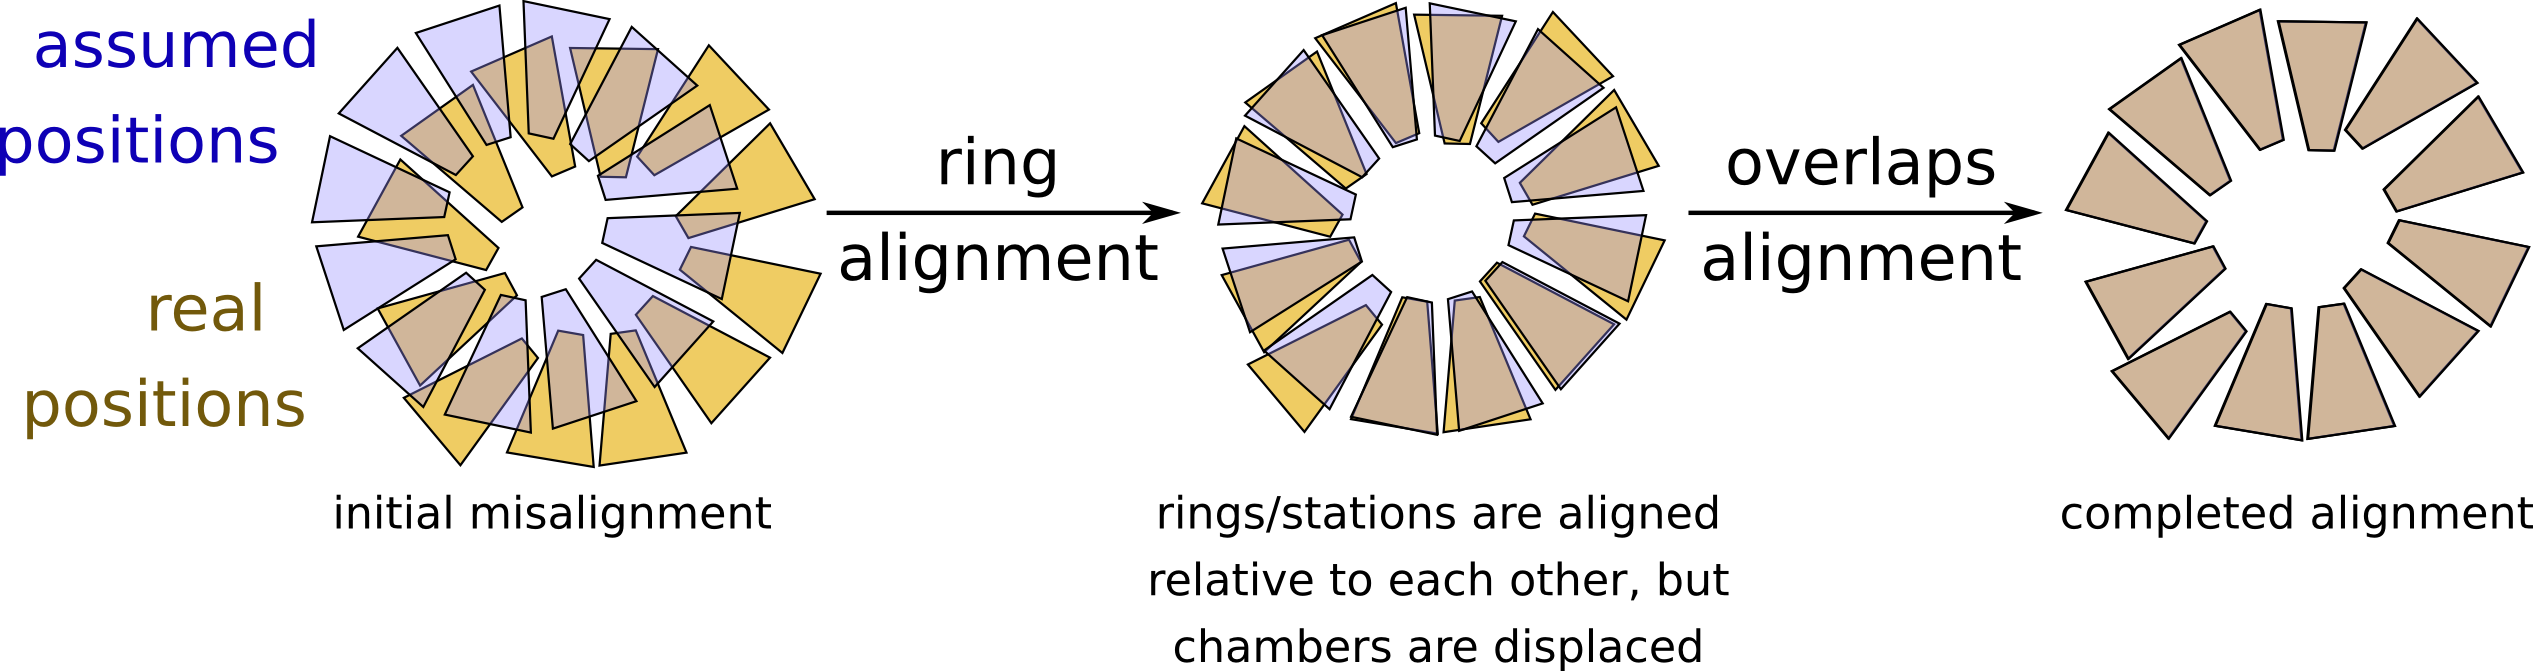
\includegraphics[width=\linewidth]{two_step_procedure.png}
\end{frame}

\vspace{0.2 cm}
\begin{frame}
\frametitle{Details of the method}

\begin{columns}
\column{0.5\linewidth}
{\small
\begin{itemize}
\item Get unbiased residuals by fitting to one chamber as a reference, aligning the other
\item Measurement propagates around the ring (in this case, to the right)
\end{itemize}
}

\column{0.5\linewidth}
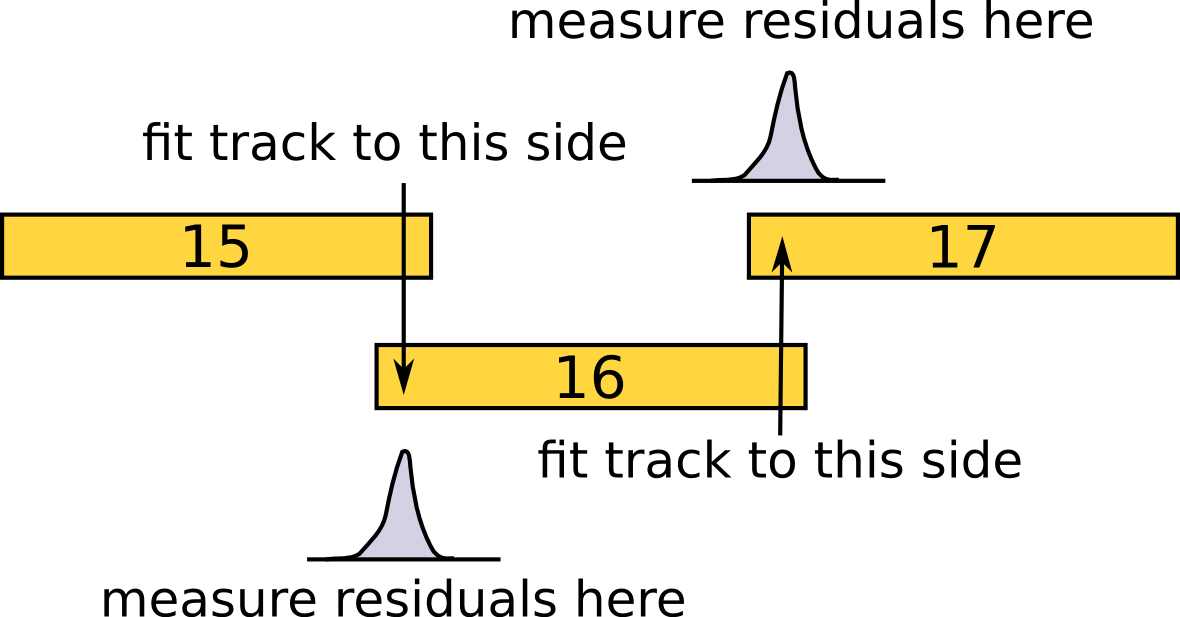
\includegraphics[width=\linewidth]{fit_to_both.png}
\end{columns}

\vspace{0.5 cm}
\hspace{-0.83 cm} \textcolor{darkblue}{\Large ME+4/1 chamber 16 in CRUZET-1}

\vspace{0.1 cm}
\hspace{0.9 cm} before quality cuts \hspace{1.7 cm} after cuts \hspace{1 cm} \mbox{after alignment\hspace{-1 cm}}

\vspace{0.1 cm}
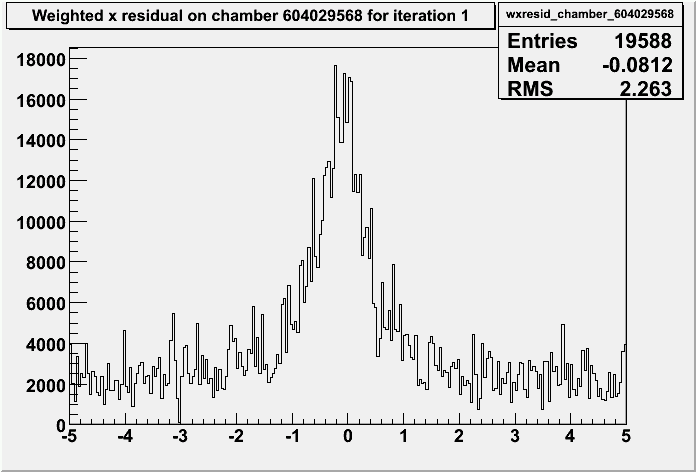
\includegraphics[height=3.5 cm]{before_cuts.png}
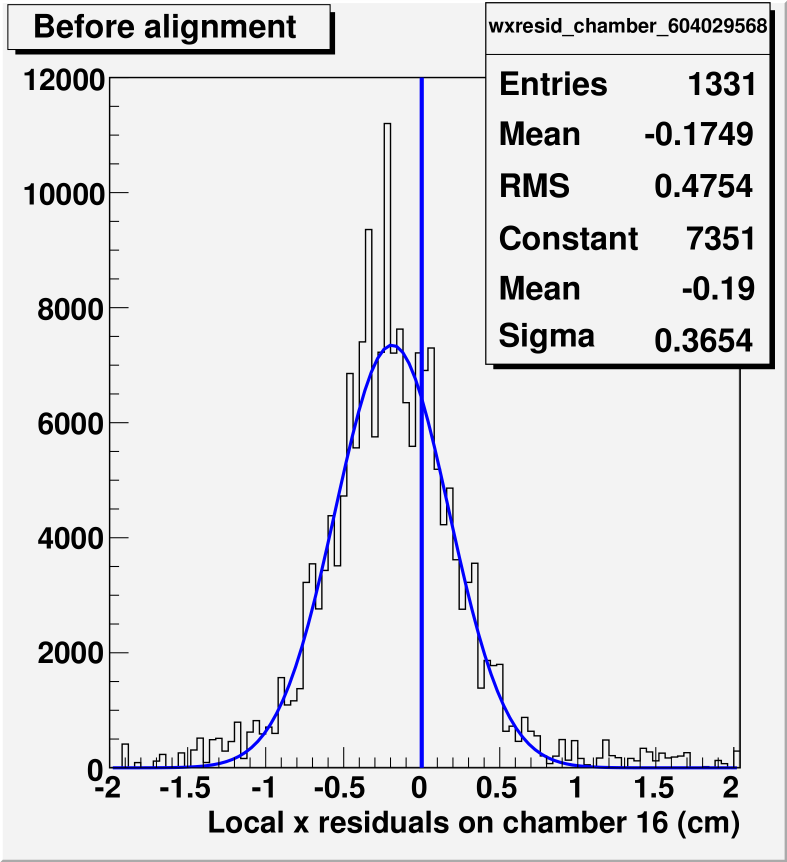
\includegraphics[height=3.5 cm]{before_alignment.png}
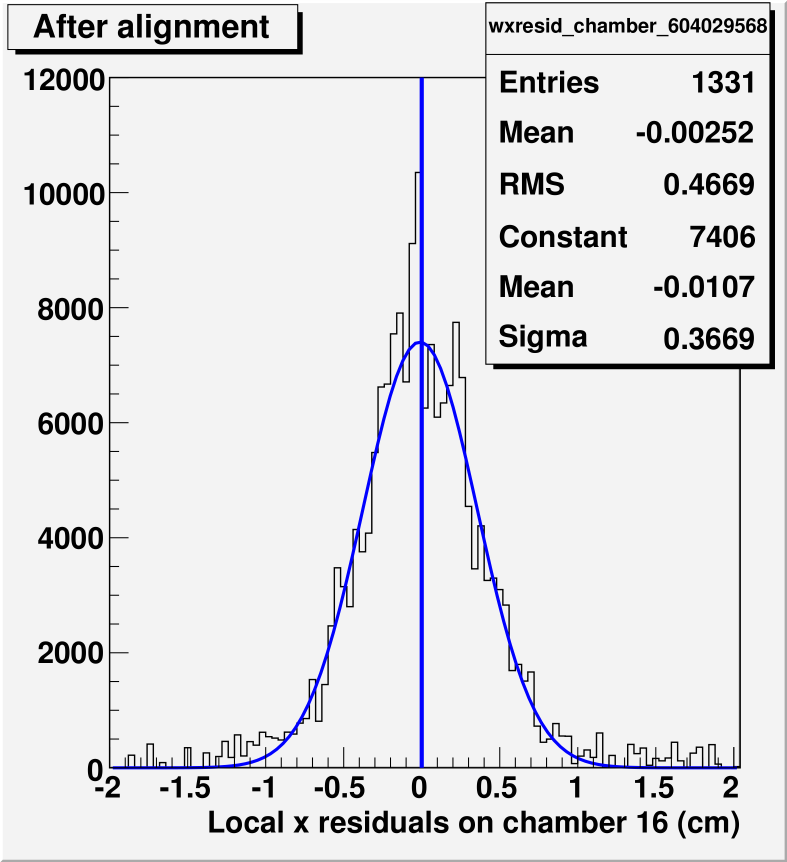
\includegraphics[height=3.5 cm]{after_alignment.png}

\end{frame}

\begin{frame}
\frametitle{Ring alignment (iteration \only<1>{1}\only<2>{2}\only<3>{3}\only<4>{4}\only<5>{5}\only<6>{6}\only<7>{7}\only<8>{8}\only<9>{9}\only<10>{10}\only<11>{11}\only<12>{12}\only<13>{13}\only<14>{14}\only<15>{15}\only<16>{16}\only<17>{17}\only<18>{18}\only<19>{19}\only<20>{20}\only<21>{21}\only<22>{22}\only<23>{23}\only<24>{24}\only<25>{25}\only<26>{26}\only<27>{27}\only<28>{28}\only<29>{29}\only<30>{30}\only<31>{31}\only<32>{32}\only<33>{33}\only<34>{34}\only<35>{35}\only<36>{36})}

\small
\hspace{-0.5 cm} ME+2/2 in CRUZET-1: \textcolor{red}{red arrows} and \textcolor{darkgreen}{green points} are \mbox{both the $r\phi$ alignment\hspace{-1 cm}}
\begin{itemize}
\item \small propagation is causal (takes exactly 35 iterations)
\item \small ring overcloses by 4~cm due to 1.2~mm systematic error
\end{itemize}

\vspace{-0.5 cm}
\begin{center}
\only<1>{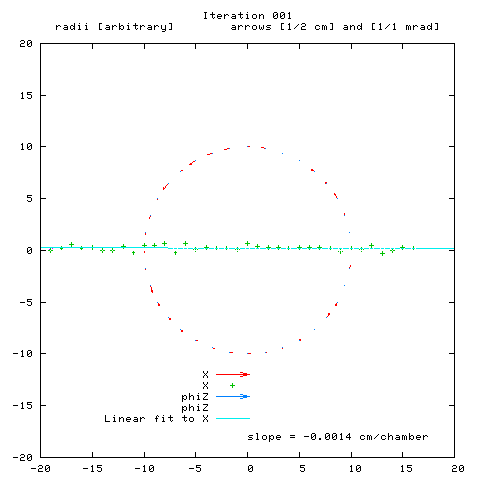
\includegraphics[height=6 cm]{frame01.png}}

\only<2>{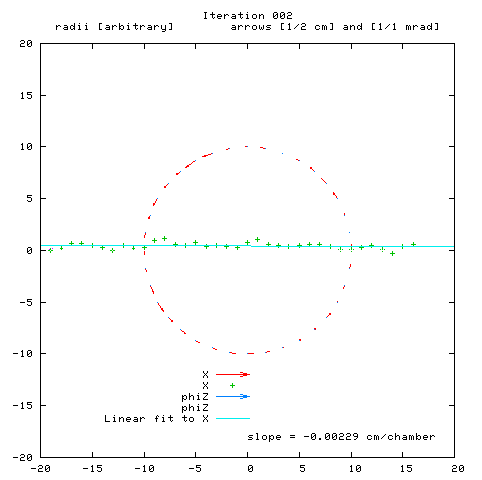
\includegraphics[height=6 cm]{frame02.png}}

\only<3>{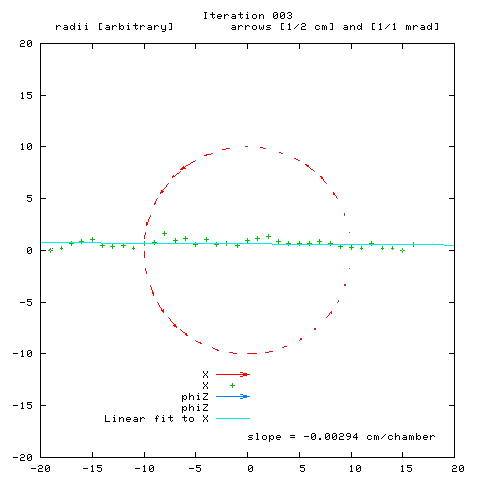
\includegraphics[height=6 cm]{frame03.png}}

\only<4>{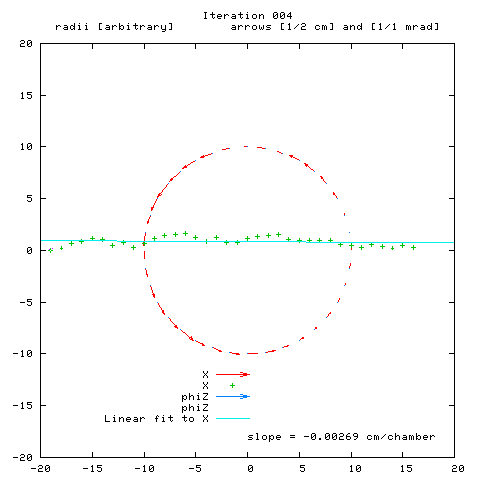
\includegraphics[height=6 cm]{frame04.png}}

\only<5>{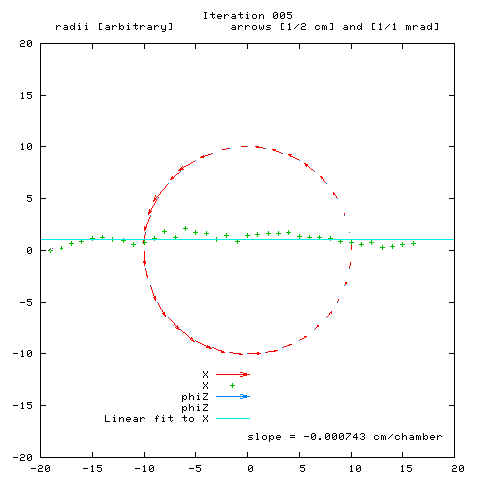
\includegraphics[height=6 cm]{frame05.png}}

\only<6>{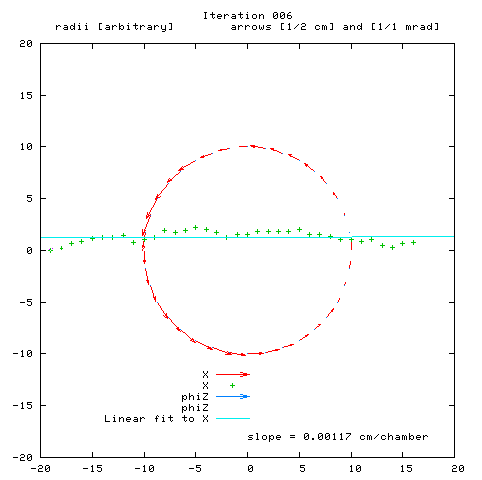
\includegraphics[height=6 cm]{frame06.png}}

\only<7>{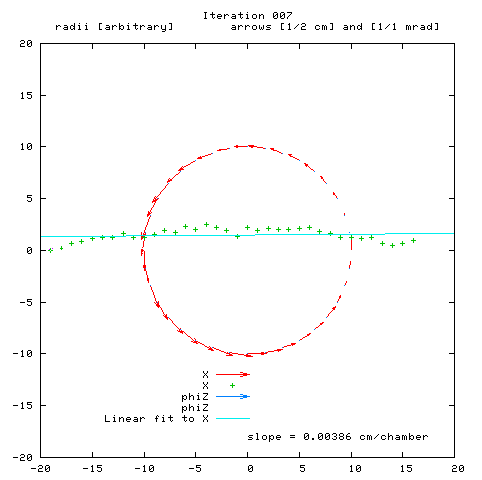
\includegraphics[height=6 cm]{frame07.png}}

\only<8>{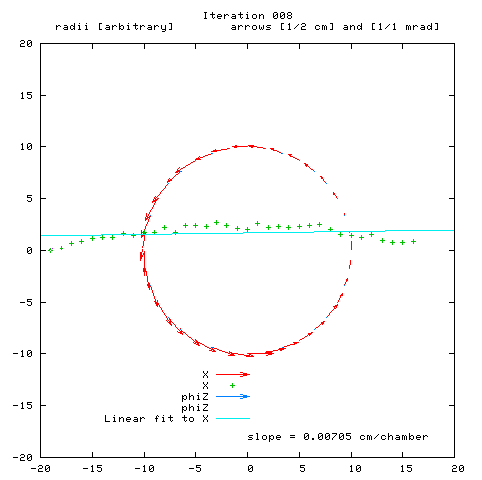
\includegraphics[height=6 cm]{frame08.png}}

\only<9>{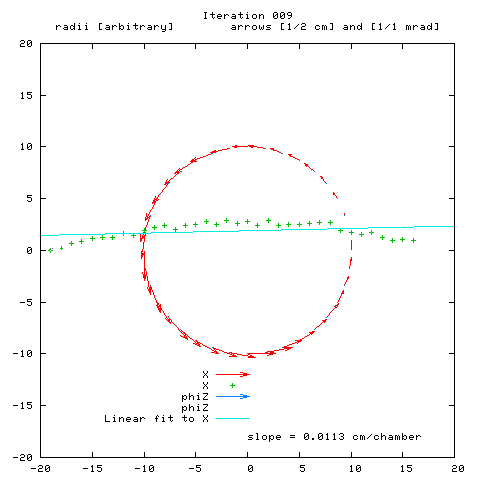
\includegraphics[height=6 cm]{frame09.png}}

\only<10>{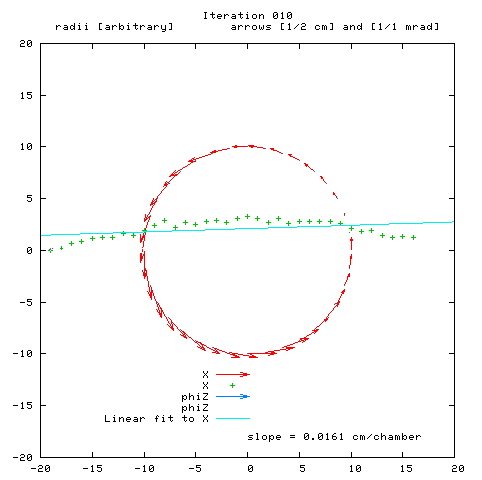
\includegraphics[height=6 cm]{frame10.png}}

\only<11>{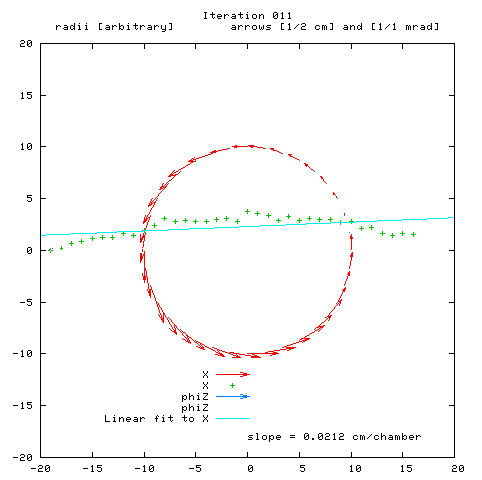
\includegraphics[height=6 cm]{frame11.png}}

\only<12>{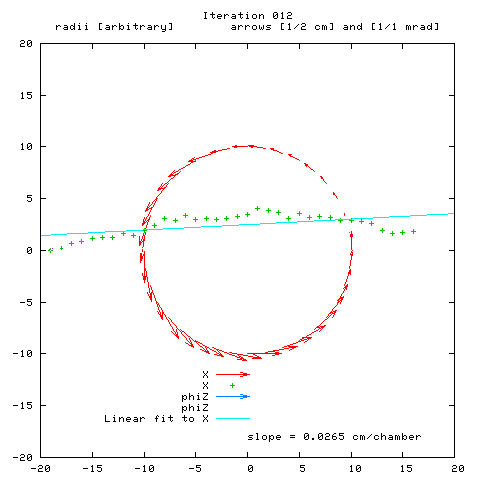
\includegraphics[height=6 cm]{frame12.png}}

\only<13>{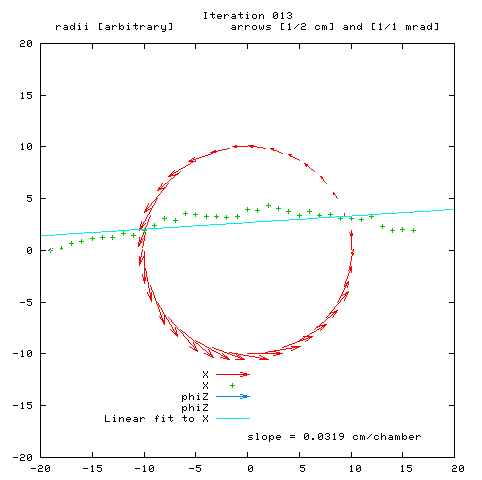
\includegraphics[height=6 cm]{frame13.png}}

\only<14>{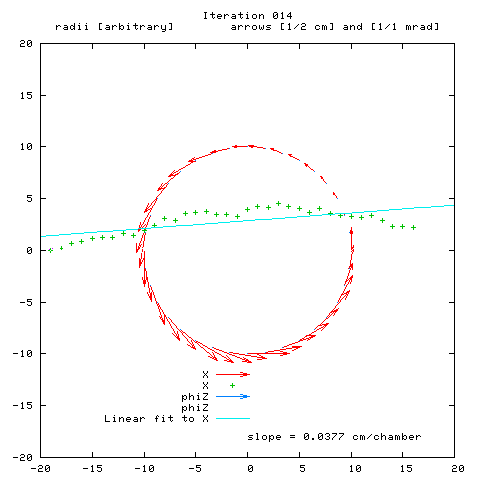
\includegraphics[height=6 cm]{frame14.png}}

\only<15>{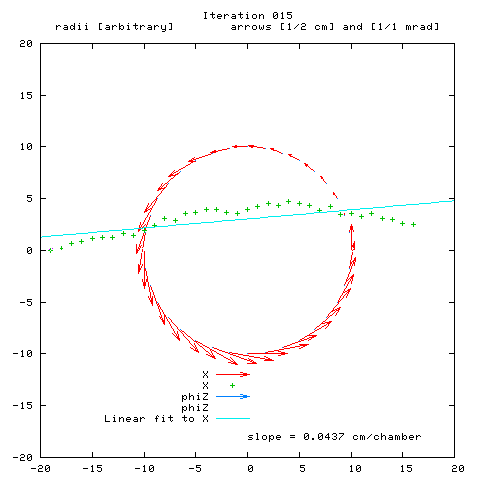
\includegraphics[height=6 cm]{frame15.png}}

\only<16>{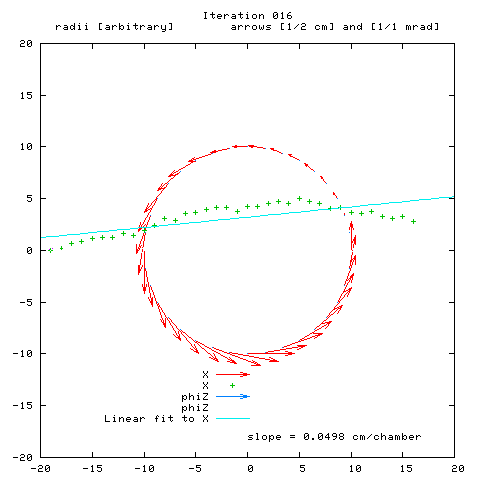
\includegraphics[height=6 cm]{frame16.png}}

\only<17>{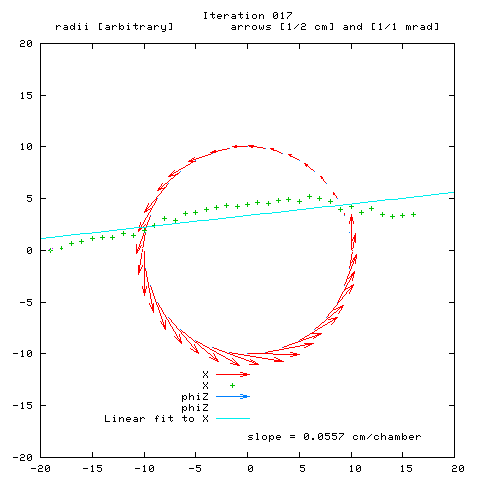
\includegraphics[height=6 cm]{frame17.png}}

\only<18>{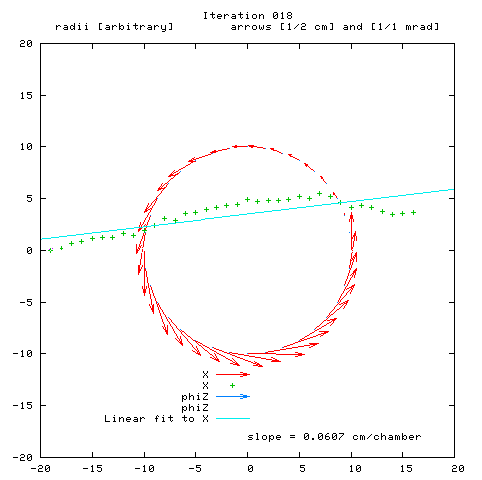
\includegraphics[height=6 cm]{frame18.png}}

\only<19>{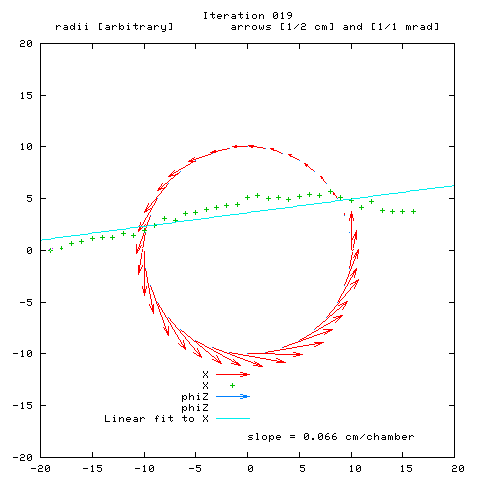
\includegraphics[height=6 cm]{frame19.png}}

\only<20>{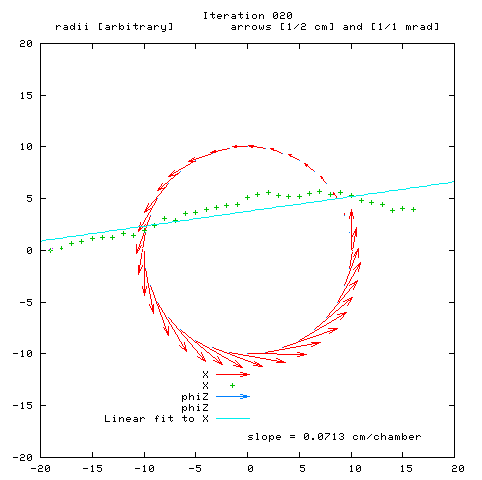
\includegraphics[height=6 cm]{frame20.png}}

\only<21>{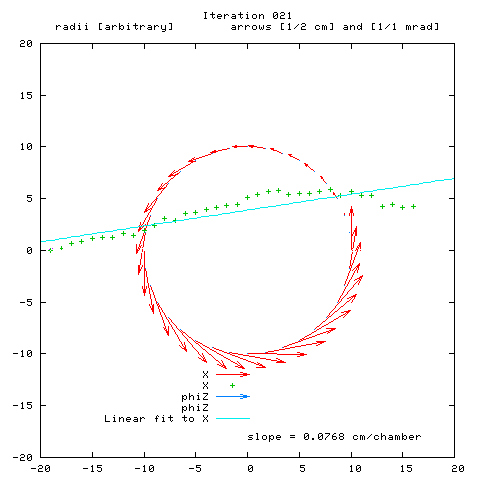
\includegraphics[height=6 cm]{frame21.png}}

\only<22>{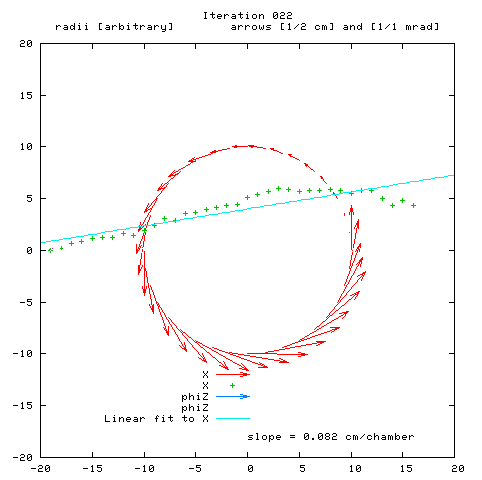
\includegraphics[height=6 cm]{frame22.png}}

\only<23>{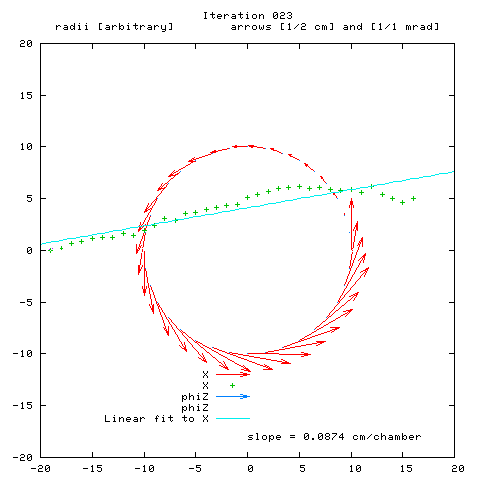
\includegraphics[height=6 cm]{frame23.png}}

\only<24>{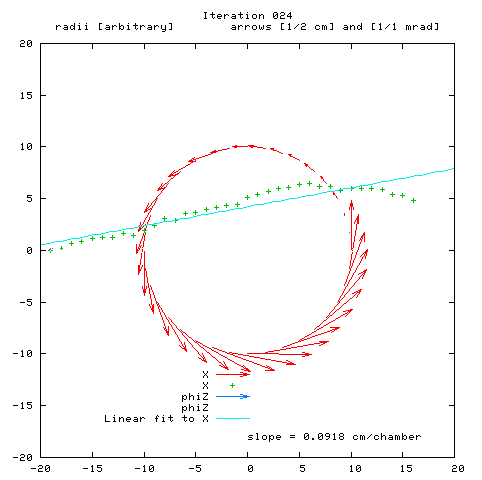
\includegraphics[height=6 cm]{frame24.png}}

\only<25>{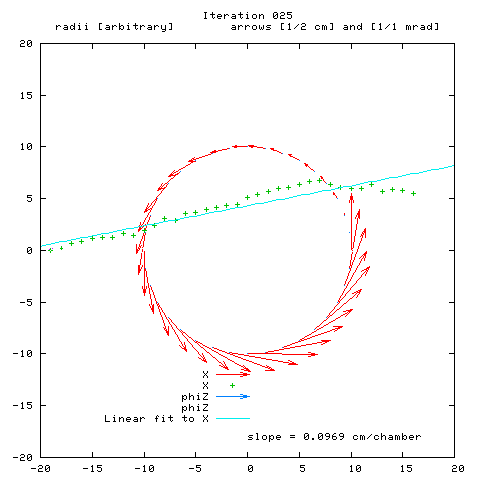
\includegraphics[height=6 cm]{frame25.png}}

\only<26>{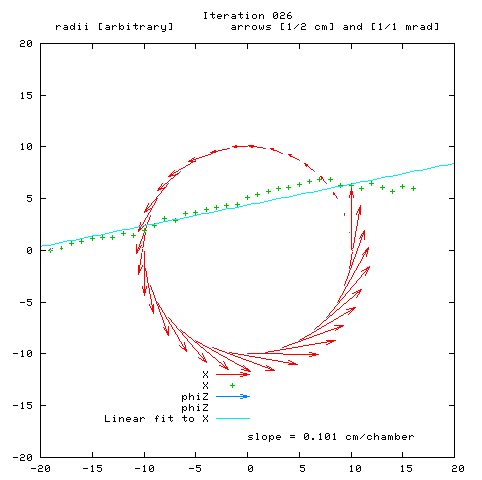
\includegraphics[height=6 cm]{frame26.png}}

\only<27>{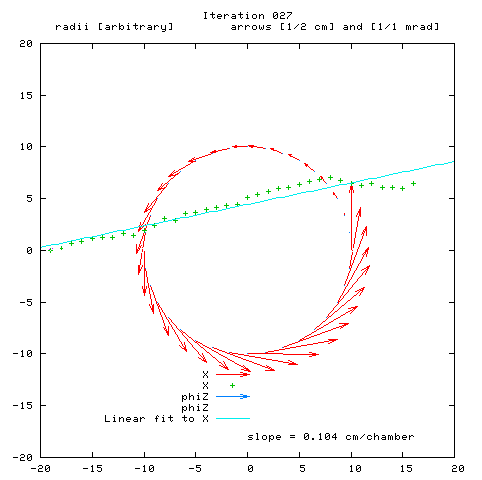
\includegraphics[height=6 cm]{frame27.png}}

\only<28>{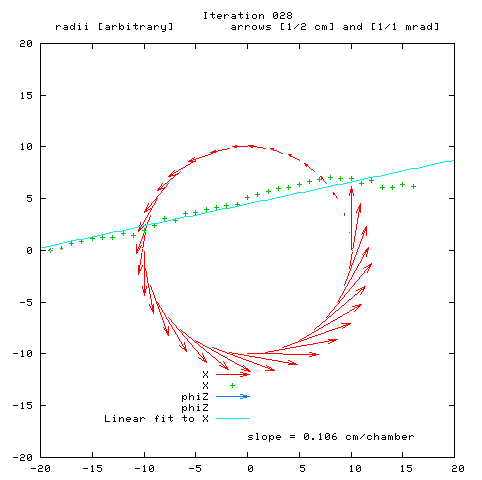
\includegraphics[height=6 cm]{frame28.png}}

\only<29>{\includegraphics[height=6 cm]{frame29.png}}

\only<30>{\includegraphics[height=6 cm]{frame30.png}}

\only<31>{\includegraphics[height=6 cm]{frame31.png}}

\only<32>{\includegraphics[height=6 cm]{frame32.png}}

\only<33>{\includegraphics[height=6 cm]{frame33.png}}

\only<34>{\includegraphics[height=6 cm]{frame34.png}}

\only<35>{\includegraphics[height=6 cm]{frame35.png}}

\only<36>{\includegraphics[height=6 cm]{frame36.png}}
\end{center}

\vspace{-1.5 cm}
\mbox{ }
\end{frame}

\begin{frame}
\addtocounter{page}{-35}
\frametitle{What's wrong?}
\small
\begin{itemize}
\item Same conclusion from CRUZET-2, including more alignment parameters, different rings (though the size of error is different)
\item Likely problem is use of $x$ residual, rather than strip $\phi$
\end{itemize}

\begin{columns}
\column{0.4\linewidth}
\mbox{ } \hfill \includegraphics[width=0.7\linewidth]{directions.png} \hfill \mbox{ }

\vspace{0.5 cm}
\includegraphics[width=\linewidth]{ignorance_of_y.png}

\column{0.65\linewidth}
\begin{itemize}
\item In our regions, $x$ has a significant component from wire measurement
\item Wire measurement is discrete due to ganging: about 3.5~cm to 5.5~cm
\item $(s,w) \to (x,y)$ transformation is an irreversible projection
\item Aligning with $s = \phi$ would require deep changes to alignment framework: we're starting with a stand-alone implementation to demonstrate the need
\item Must modify track-fits as well (also restricted to the edges)
\end{itemize}
\end{columns}
\end{frame}

\begin{frame}
\frametitle{How does this effect work?}

\begin{columns}
\column{0.5\linewidth}
\includegraphics[width=\linewidth]{vertical_residual.png}

\column{0.5\linewidth}
\includegraphics[width=\linewidth]{selectioneffect_nocut.pdf}

\end{columns}

\vfill
\begin{itemize}
\item Asymetric coverage can introduce fake ``misalignments'' on the order of several millimeters
\item Effect would be the same in every chamber of a given ring, leading to exactly the lack of closure we saw
\end{itemize}
\end{frame}

\begin{frame}
\frametitle{Debugging geometry}
\small

\vfill
While trying to resolve the overclosure problem, we found two errors
in the software description of the detector, relative to integration
drawings.  Thanks to Tim, Oleg, and Richard!

\vfill
\begin{columns}
\column{0.5\linewidth}
\hfill \includegraphics[width=0.85\linewidth]{expand_ME22_32.png}

\column{0.6\linewidth}
\includegraphics[width=0.85\linewidth]{move_all_pins.png}
\end{columns}

\vfill 
\begin{columns}
\column{0.5\linewidth}
\textcolor{darkblue}{\Large Revised strategies}

\begin{itemize}
\item strip $\to$ $\phi$ is simplest
\item 1-D alignments can only use hits on one side (convergence)
\item can get 2-D from strips alone
\end{itemize}

\column{0.5\linewidth}
\includegraphics[width=\linewidth]{revised_strategy.png}
\end{columns}
\end{frame}

\begin{frame}
\frametitle{Conclusions for CSC-Overlaps}
\begin{itemize}\setlength{\itemsep}{0.75 cm}
\item Surprisingly, this the most challenging alignment procedure
  (including some reasons not described here)
\item When the chambers are so close, they ``see'' the fine-grain
  details of their neighbors, some of which can cause biases
\item We're modifying the procedure to access the strip data directly
  for both the track-fits and the hit residuals
\end{itemize}
\end{frame}

\section*{Conclusions}

\begin{frame}
\frametitle{Final conclusions:}

\vspace{-0.35 cm}
\hspace{-0.83 cm} \textcolor{darkblue}{\Large Are we ready for data-taking?}

\vfill
\begin{itemize}\setlength{\itemsep}{0.25 cm}
\item Long-term procedure is well-established: it will provide
  an alignment of a half-millimeter or better when it's first needed
  for physics studies: $\sim$10~pb$^{-1}$

\item Our tools are flexible enough to develop a station-finding
  algorithm in a matter of days, allows us to think on our feet and
  respond to what the data tell us

\item Station alignment satisfies internal consistency checks, makes
  sense, agrees with external information where available:

I submit that it is correct (can anyone prove me wrong?)

\item CSC-Overlaps procedure is subtle because it looks at hits
  under a microscope.  Once we solve the edge-effect type problems, it
  will be a precise technique.

\vfill Hopefully, we'll have lots of beam-halo! (That we can use!)

\end{itemize}
\label{numpages}
\end{frame}

\end{document}
